\documentclass[11pt,oneside,a4paper]{report}


% Packages to use
\usepackage{graphicx}
\usepackage{hyperref}
\usepackage{amsmath}
\usepackage{amssymb}
\usepackage{amstext}
\usepackage{amsthm}
\usepackage{palatino}
\usepackage[a4paper]{geometry}
\usepackage[dvips]{color}
\usepackage[toc,page]{appendix}
\usepackage{sectsty}
\usepackage{subfigure}
\usepackage{natbib}

% TODO Lav theoremstyle så den er ordenlig!
\newtheoremstyle{mystyle}% ⟨name⟩ 
{5pt}%	⟨Space above⟩ 
{25pt}%	⟨Space below⟩ 
{}%	⟨Body font⟩
{\parindent}%	⟨Indent amount⟩
{\bfseries}% ⟨Theorem head font⟩ 
{:}%	⟨Punctuation after theorem head⟩ 
{.5em}%	⟨Space after theorem head⟩
{}%	⟨Theorem head spec (can be left empty, meaning ‘normal’)⟩

\theoremstyle{mystyle}
\newtheorem{definition}{Definition}[section]
\newtheorem{example}{Example}[section]
\newtheorem{convention}{Convention}[section]
\newtheorem{lemma}{Lemma}[section]


\title{Visualization of $\beta$-reduction-graphs in the lambda calculus}
\author{Niels Bjørn Bugge Grathwohl & Jens Duelund Pallesen}
\date{\large \today}


%  New color
\definecolor{sectionColor}{RGB}{65,117,78}


% Color & size for sections
\chapterfont{\Huge\color{sectionColor} }
\sectionfont{\large\color{sectionColor} }
\subsectionfont{\Small\color{sectionColor} }


% Margins
\geometry{top=2.0cm, bottom=2.0cm, left=2.0cm, right=2.0cm}


\newcommand{\Z}{\mathbb{Z}}
\newcommand{\R}{\mathbb{R}}
\newcommand{\N}{\mathbb{N}}
\newcommand{\lam}[2]{\lambda#1.#2}
\newcommand{\BETA}{\boldsymbol\beta}
\newcommand{\barrow}{\rightarrow_\beta}
\newcommand{\Barrow}{\barrow^*}
\newcommand{\I}{\textsf{\textbf{I}}}
\newcommand{\W}{\textsf{\textbf{W}}}

% Bruges til Python-kode.
\newcommand{\pycode}[1]{\texttt{#1}}


%%%%%%%%%%%%%%%%%%%%%%%%%%%%%%%%%%%%%%%%%%%%%%%%%%
\begin{document}
%%%%%%%%%%%%%%%%%%%%%%%%%%%%%%%%%%%%%%%%%%%%%%%%%%

% Title page
% %!TEX root = rapport.tex

\begin{titlepage}


% Front page image
\begin{flushright}
	
\includegraphics[scale=0.5]{images/titleLogo.png}\\[2.0cm]
\end{flushright}

\begin{center}

% Title
\textcolor{sectionColor}{{\huge \bfseries Visualization of $\beta$-reduction-graphs in the lambda calculus}\\[2.0cm]}
% Author and supervisor
\begin{minipage}{0.4\textwidth}
\begin{flushleft} \large
\emph{Author:}\\
Niels Bj\o rn Bugge Grathwohl\\
Jens Duelund Pallesen
\end{flushleft}
\end{minipage}
\begin{minipage}{0.4\textwidth}
\begin{flushright} \large
\emph{Supervisor:} \\
Jakob Grue Simonsen
\end{flushright}
\end{minipage}
 
\vfill
 
% Bottom of the page
{\large \today}
 
\end{center}
 
\end{titlepage}

% Abstract
% %!TEX root = rapport.tex

\begin{abstract}

\textbf{Background} This is a project in how to visualize reduction graphs in
the lambda calculus. It is a part of the master education in Computer Science
at the University of Copenhagen. Our focus in this project is to implement a
piece of software in Python, that can visualize reduction graphs in a
``pretty'' and informative way. The target group for the project is
theoretical computer scientists with an interest in the lambda calculus. We
will, besides Python implementation, work with both general lambda calculus
theory and visualization / graph theory.

\textbf{Results} Our results are...

\textbf{Conclusion} The conclusion is...

\end{abstract}

% Table of content
% \tableofcontents
%\listoftables
%\listoffigures
%\newpage
%
% Chapters
%!TEX root = rapport.tex

\chapter{Introduction}

We will in this project develop an automatic method for visualization of 
$\beta$-reduction graphs of lambda terms. The method has been implemented in 
the programming language Python.

Until now there did not exist any software for reduction graph visualization.
Researchers wanting to visualize reduction graphs have therefore been limited
to either their own drawings or to what they can imagine. Since reduction
graphs can be very large, this posed a very tight constraint on what could be
visually presented. 

In our opinion, software for this visualization task presents two primary
challenges: The drawn graphs must be \emph{informative} and
\emph{good-looking}. These two matters are not entirely independent of each
other; very often the particular layout of a graphs two-dimensional embedding
greatly reduces clutter and ``noise'', thus adding information. The opposite
can of course also be the case, which is why the two problems are
interchanged.

The intended user of the software is a theoretical computer scientist that
does research in the field of lambda calculus. Our hope is that researchers
can use this tool to gain new insight into the lambda calculus, and that it
will serve as a source of inspiration for new research because it offers a new
look at a well-known concept.

% \section{Project constraints \& risks}
% Because reduction graphs very often tend to become huge, there arises the
% problem of deci ding whether they can be drawn on a plane at all. We will
% perhaps have to develop a routine for deciding this, along with routines for
% reordering the graph. Alternatively, a set of ``best practices'' for drawing
% the nodes could be developed that would minimize the amount of crossing edges
% as the film progresses forward. Yet more alternatively, methods for 3D-drawing
% could be considered. However, this will demand great care when determining the
% look of the images, as a 3-dimensional rendering of a large graph very easily
% could inhibit understanding and confuse the beholder, which is the opposite of
% what we are working towards.
% 
% Furthermore, there is a design choice to be made whether each frame of the
% film should be drawn immediately after the reduction step has been completed,
% making the film rendering and the term reductions synchronized, or whether the
% rendering should begin only after all desired (or possible) reductions have
% been computed.

%!TEX root = rapport.tex

\chapter{Project constraints \& risks}
Because reduction graphs very often tend to become huge, there arises the
problem of deciding whether they can be drawn on one plane at all. The
development of a routine for deciding this, along with routines for reordering
the graph could be the solution for this. Alternatively, a set of ``best
practices'' for drawing the nodes could be developed that would minimize the
amount of crossing edges as the film progresses forward. Yet more
alternatively, methods for 3D-drawing could be considered. However, this will
demand great care when determining the look of the images, as a 3-dimensional
rendering of a large graph very easily could inhibit understanding and confuse
the beholder, which is the opposite of our goal.
%!TEX root = rapport.tex

\chapter{Preliminaries: Basic Lambda Calculus}

% The untyped lambda calculus was introduced in 1936 by Alonzo Church
% [reference] as part of the search for a solid foundation for mathematics. It is
% heavily intertwined with the notion of a ``function'', in the sense that logic
% and mathematics is represented with only functions and untyped variables that
% can be either free or bound.


% alt er funktioner
% eksempler

As a very informal example, here is a function that doubles an integer:
\begin{equation*}
	(\lam{x}{x+x})2=4.
\end{equation*}
This example shows a \emph{bound variable}, $x$, and an implicit \emph{reduction step}. The variable $x$
is said to be bound because the lambda function uses it as an argument. Contrast this to
\begin{equation*}
	(\lam{x}{x+y})2=2+y.
\end{equation*}
Here, $y$ is a variable that has no values assigned to it yet. From
the context we can say nothing about $y$, so we give it the predicate
``free''. In this second example there was yet another reduction step, which 
can be regarded as a rewriting action on the string representing the
lambda term. More informally, one can think of it as ``substituting in''
the values for the bound variables. In the examples above this amounts to
replacing $x$ with the number 2.

% definition af syntax
\section{Syntax}
\begin{definition}
	The lambda calculus consists of \emph{lambda terms} defined over the alphabet:
	\begin{align*}
		x,y,z,\hdots\ &\in V\\
		\lambda\ &\text{ abstractor} \\
		()\ &\text{ parentheses}
	\end{align*}
	where $V$ is the countable, infinite set containing variable names $v_0,v_1,v_2,\hdots$.
	The set of all lambda terms $\Lambda$ is defined inductively as follows:
	\begin{align*}
		x\in\Lambda \\
		M\in\Lambda &\Rightarrow (\lam{x}{M})\in\Lambda \\
		M, N\in\Lambda &\Rightarrow (M N)\in\Lambda
	\end{align*}
where $x\in V$.
\end{definition}
\begin{convention}
	A term $\lam{x}{M}$ is called a function.
\end{convention}
\begin{convention}
	For brevity, we leave out the outermost parentheses.
\end{convention}
\begin{convention}
	Evaluation is left associative:
	\begin{equation*}
		M N P \equiv (M N) P
	\end{equation*}
\end{convention}
\begin{convention}
	Function bodies extend as far as possible:
	\begin{equation*}
		\lam{x}{M N}\equiv\lam{x}{(M N)}\not\equiv(\lam{x}{M})N
	\end{equation*}
\end{convention}
\begin{convention}
	Functions take exactly one argument, but as syntactic sugar we use:
	\begin{equation*}
		\lam{xy}{xy}\equiv\lam{x}{\lam{y}{xy}}
	\end{equation*}
\end{convention}

\section{Free Variables}

As already indicated, the variables in a lambda term can be divided into
two groups; the free and the bound variables.

\begin{definition}
	The set $FV(M)$ is the smallest set containing all free variables of the lambda
	term $M$, defined by:
	\begin{align*}
		FV(x)&=\{x\} \\
		FV(\lam{x}{M})&= FV(M) - \{x\} \\
		FV((M N)) &= FV(M) \cup FV(N)
	\end{align*}
\end{definition}
\begin{definition}
	\begin{enumerate}
		\item If $FV(M)=\emptyset$, $M$ is said to be \emph{closed}.
		\item The set of all closed terms is denoted $\Lambda^0$.
	\end{enumerate}
\end{definition}
\begin{definition}
	A variable $x$ that is not free is \emph{bound}.
\end{definition}

\section{Substitution}

It is possible to substitute
values for free variables. These values are not limited to being just new
variables, but can be any lambda term. A substitution is notated:
\begin{align*}
	M[x:=N]
\end{align*}
with the intuitive meaning that all free occurences of $x$ are replaced with 
the term $N$.
\begin{definition}
Substitution is defined as follows (\cite{Barendregt} 2.1.15):
\begin{align*}
	x[x:=N]&\equiv N \\
	y[x:=N]&\equiv y, \text{ if } x \not\equiv y \\
	(\lam{y}{M})[x:=N]&\equiv\lam{y}{(M[x:=N])}, \text{ if } x\not\equiv y \\
	(\lam{x}{M})[x:=N]&\equiv\lam{x}{M} \\
	(M L)[x:=N]&\equiv(M[x:=N])(L[x:=N])
\end{align*}
\end{definition}
Using this definition, the following result can be shown (\cite{Barendregt} p. 28):
\begin{lemma}\label{lem:subst}
	\begin{enumerate}
		\item $M=M'\Rightarrow M[x:=N]=M'[x:=N]$.
		\item $N=N'\Rightarrow M[x:=N]=M[x:=N']$.
		\item $M=M', N=N'\Rightarrow M[x:=N]=M'[x:=N']$.
	\end{enumerate}
\end{lemma}
Lemma \ref{lem:subst} tells us, informally, that the meaning of a a lambda term
is closed under substitution with equals.

\section{Subterms}

A lambda term $M$ is composed of several parts which we call \emph{subterms}.
\begin{definition}
	\begin{enumerate}
		\item $N\subset M$ denotes that $N$ is a subterm of $M$. The set $Sub(M)$ is the 
		smallest set such that all subterms of $M$ are contained in $Sub(M)$:
		\begin{align*}
			Sub(x) &=\{x\} \\
			Sub(\lam{x}{N}) &= Sub(N) \cup \{\lam{x}{N}\} \\
			Sub(M N) &= Sub(M) \cup Sub(N) \cup Sub(M N)
		\end{align*}
		\item A subterm $N$ of $M$ is called \emph{active} if $N L \subset M$ 
		for a term $L$ and \emph{passive} otherwise.
	\end{enumerate}
\end{definition}
\begin{example}\label{exmpl:subterms}
	The term $M\equiv\lam{x}{xy(\lam{z}{y})}$ has the following subterms:
	\begin{itemize}
		\item $\lam{x}{((xy)(\lam{z}{y}))}\subset M$, passive.
		\item $(xy)(\lam{z}{y})\subset M$, passive.
		\item $xy\subset M$, active.
		\item $\lam{z}{y}\subset M$, passive.
		\item $x\subset M$, active.
		\item $y\subset M$, passive.
	\end{itemize}
\end{example}
Note that the subterm $y$ occurs two times in Example \ref{exmpl:subterms}.

\section{$\alpha$-congruence}

The particular name of a bound variable does not affect the function represented 
by a lambda term. Thus, the two terms
\begin{align*}
	\lam{x}{x} \\
	\lam{y}{y}
\end{align*}
denote the same function, namely the identity. This gives rise to a definition of congruence
that is essential in the lambda calculus.
\begin{definition}
	\begin{enumerate}
		\item For a term $M$, \emph{change of bound variables} is defined as a substitution
		of a part of $M$, $\lam{x}{N}$, with $\lam{y}{N[x:=y]}$, i.e. all occurences of $x$
		are replaced with an occurence of $y$. It is a requirement that $y$ does not 
		occur in $N$.
		\item $M$ and $N$ are $\alpha$-congruent, $M\equiv_\alpha N$, if $N$ is the
		resulting term after a finite sequence of changes of bound variables in $M$.
	\end{enumerate}
\end{definition} 
For instance, we have:
\begin{example}
\begin{align*}
	\lam{x}{x}&\equiv_\alpha\lam{y}{y} \\
	\lam{x}{\lam{y}{xy}}&\equiv_\alpha{\lam{a}{\lam{b}{ab}}} \\
	\lam{x}{\lam{y}{xy}}&\not\equiv_\alpha\lam{y}{\lam{y}{yy}}
\end{align*}
\end{example}
This last example illustrates the need for the requirement that $y$ cannot
occur in $N$. In the following we will regard $\alpha$-congruent terms as
being equivalent, so the notation $\equiv$ is used instead of
$\equiv_\alpha$.

\section{Contexts}

\begin{definition}
	\begin{enumerate}
		\item A context $C[\ ]$ is an ``unfinished term'' with holes in it. 
		\item The set $Con$ contains all contexts and is defined as the smallest
		set satisfying these constraints:
		\begin{align*}
			[\ ]&\in Con \\
			M\in\Lambda\Rightarrow M[\ ]&\in Con \\
			M\in\Lambda\Rightarrow [\ ]M&\in Con \\
			C\in Con\Rightarrow C[\ ]&\in Con \\
			C\in Con\Rightarrow [\ ]C&\in Con
		\end{align*}
		\item Terms can be plugged into the holes, thus completing the term. 
		\item When plugging a term into a hole, we do not work modulo 
		$\alpha$-congruence.
	\end{enumerate}
\end{definition}
\begin{example}
	Given the context $C[\ ]\equiv\lam{x}{x[\ ]}$, we can make new lambda terms:
	\begin{align*}
		C[x]&\equiv\lam{x}{xx} \\
		C[\lam{y}{y}]&\equiv\lam{x}{x\lam{y}{y}}
	\end{align*}
\end{example}

\section{$\beta$-reduction}

In this section we shall define a key concept of the lambda calculus which
plays a central role in this report, namely the $\beta$-reduction. This
reduction captures the notion of ``substituting in'' terms for bound variables,
and can be intuitively thought of as ``solving'' a lambda term by reducing it
to a (sometimes) simpler form.

\begin{definition}\label{def:betareduction}
	\begin{enumerate}
		\item \emph{$\beta$-reduction} is a binary relation $\BETA\subseteq\Lambda^2$ such that
		\begin{equation*}
			\BETA=\Big\{\big((\lam{x}{M})N,\ M[x:=N]\big)\big|M,N\in\Lambda\Big\}.
		\end{equation*}
		\item For an element $(M,N)\in\BETA$ we call $M$ a \emph{$\beta$-redex} and
		$N$ a \emph{$\beta$-contractum} of $M$.
		\item A term $M$ is in \emph{$\beta$-normal-form} ($\beta$-nf) if it 
		does not contain any subterms that are $\beta$-redexes.
	\end{enumerate}
\end{definition}
\begin{definition}
	Definition \ref{def:betareduction} is extended up to contexts.
	\begin{align*}
		C\big[(\lam{x}{M})N\big]\equiv C\big[M[x:=N]\big]
	\end{align*}
\end{definition}
\begin{definition}\label{def:beta_rel1}
	We have the relations (\cite{Barendregt} def. 3.1.5]):
	\begin{align*}
		(M,N)\in\BETA&\Rightarrow M\barrow N \\
		M\barrow N &\Rightarrow ZM\barrow ZN \\
		M\barrow N &\Rightarrow MZ\barrow NZ \\
		M\barrow N &\Rightarrow \lam{x}{M}\barrow \lam{x}{N} 
	\end{align*}	
\end{definition}
\begin{definition}\label{def:beta_rel2}
	The transitive, reflexive closure of $\barrow$ is notated $\Barrow$:
	\begin{align*}
		M\barrow N &\Rightarrow M\Barrow N \\
		M\Barrow N, N\Barrow L &\Rightarrow M\Barrow L \\
		M\Barrow M & 
	\end{align*}
\end{definition}
\begin{definition}
	The relations from Definitions \ref{def:beta_rel1} and \ref{def:beta_rel2} 
	generate an equivalence relation:
	\begin{align*}
		M\Barrow N &\Rightarrow M=_\beta N \\
		M=_\beta N &\Rightarrow N=_\beta M \\
		M=_\beta N\wedge N=_\beta L&\Rightarrow M=_\beta L
	\end{align*}	
\end{definition}
\begin{definition}
	A term $N$ is a \emph{$\beta$-normal form of $M$} if $M=_\beta N$ and $N$ is in $\beta$-normal form.
\end{definition}
\begin{definition}
	For two terms, $M\Barrow N$, we call $N$ the \emph{reduct} of $M$.
\end{definition}
From these definitions it follows (\cite{Barendregt} 3.1.10), that if $M$ is a
$\beta$-nf then $\neg\exists N:M\barrow N$ and $M\Barrow N\Rightarrow M\equiv N$.

The following example from \cite{Barendregt} p. 52 illustrates the concept:
\begin{example}
	$(\lam{x}{xx})(\lam{y}{y})z\Barrow z$, and hence $(\lam{x}{xx})(\lam{y}{y})z =_\beta z$.
	More elaborately:
\begin{align*}
	(\lam{x}{xx})(\lam{y}{y})z&\barrow(\lam{y}{y})(\lam{y}{y})z \\
	&\barrow(\lam{y}{y})z \\
	&\barrow z
\end{align*}
\end{example}

% Skal der være noget om kontekster?

\section{Reduction Graphs}

When a $\beta$-redex $M$ contains subterms $\Delta_{0\hdots n}$ that are themselves 
$\beta$-redexes, an ambiguity concerning the order of $\beta$-reductions arises.
Consider the following example from \cite{Barendregt} 3.1.19:
\begin{example}
	Let $M\equiv(\lam{x}{xx})\Delta$ and $\Delta\barrow\Delta'$. We can then perform the two reductions:
\begin{align*}
	M&\barrow(\lam{x}{xx})\Delta' \\
	M&\barrow\Delta\Delta
\end{align*}
\end{example}
The example shows that we can choose to reduce $\Delta$ to its contractum $\Delta'$, or
we can choose to reduce $M$ to its contractum $\Delta\Delta$. This is notated as 
$\overset{\Delta}\barrow$ and $\overset{M}\barrow$ respectively. Different
subterms can have the same contractum, as this example illustrates:
\begin{example}
	Let $\I\equiv\lam{x}{x}$. Then:
\begin{align*}
	\I(\I x)&\overset{\I x}\barrow\I x \\
	\I(\I x)&\overset{\I(\I x)}\barrow\I x
\end{align*}
\end{example}
The set of reductions from a redex $M$ can
be considered as a directed graph, with each arc going out of a node representing
a reduction on some subterm of that node, and each node representing a lambda term that
is the contractum of the terms represented by the nodes parents.
\begin{definition}
	The \emph{$\beta$ reduction graph} of $M$, written $G_\beta(M)$, consists
	of the nodes in the set $V$ and the arcs in the multiset $A$. The set
	of nodes and multiset of arcs in $G_\beta(M)$ are defined as:
\begin{align*}
	V&=\{N\in\Lambda|M\Barrow N\} \\
	A&=\{(N_0, N_1)\in\Lambda^2|N_0,N_1\in V\wedge N_0\barrow N_1\}
\end{align*}
	Since $A$ can contain duplicates it follows that if there are more than one
	different reduction step from $N_0$ to $N_1$, that many arcs will be included 
	in $G_\beta(M)$.
\end{definition}
\begin{example}
	\begin{enumerate}
		\item The reduction graph illustrated in Figure \ref{fig:images_graphs_graf2}
		for the term $\I x$, $G_\beta(\I x)$, with
		the previous definition of $\I$ captures the reduction $\I x\barrow x$.
		
		\item $G_\beta(\I(\I x))$ is illustrated in Figure \ref{fig:images_graphs_graf1}.
		
		\item Let $\Omega\equiv(\lam{x}{xx})(\lam{x}{xx})$. $G_\beta(\Omega)$
		can be seen in Figure \ref{fig:images_graphs_graf3_omega}.
		
		\item Let $\W\equiv\lam{xy}{xyy}$. $G_\beta(\W\W\W)$ is illustrated in
		Figure \ref{fig:images_graphs_graf4_www}.
		
		\item Let $M\equiv\lam{x}{(\lam{y}{yy})x}$. $G_\beta(MM)$ is pictured in
		Figure \ref{fig:images_graphs_graf5_MM}.
		
		\item Let $w_3\equiv\lam{x}{xxx}$. Figure \ref{fig:images_graphs_graf6_w3w3}
		contains the reduction graph. Note that this graph contains an infinite 
		amount of nodes and arcs.
		
		\item In Figure \ref{fig:images_graphs_graf7_omega_w3} there is another
		example of a graph containing an infinite amount of nodes and arcs. This
		graph captures qualities found in the two graphs $G_\beta(\Omega)$ and
		$G_\beta(w_3w_3)$.
	\end{enumerate}
	\begin{figure}[htbp]
		\centering
		\begin{tabular}{ccc}
			\subfigure[$G_\beta(\I x)$]{
				
\includegraphics{../images/graphs/graf2.png}
				\label{fig:images_graphs_graf2}
			} &
			\subfigure[$G_\beta(\I(\I x))$]{
				
\includegraphics{../images/graphs/graf1.png}
				\label{fig:images_graphs_graf1}
			} & 
			\subfigure[$G_\beta(\Omega)$]{
				
\includegraphics{../images/graphs/graf3_omega.png}
				\label{fig:images_graphs_graf3_omega}
			} \\ \\
			\subfigure[$G_\beta(\W\W\W)$]{
				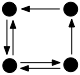
\includegraphics{../images/graphs/graf4_www.png}
				\label{fig:images_graphs_graf4_www}
			} \hspace{1.5em}
			&
			\subfigure[$G_\beta(MM)$]{
				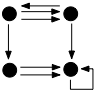
\includegraphics{../images/graphs/graf5_MM.png}
				\label{fig:images_graphs_graf5_MM}
			}\hspace{1.5em}
			&
			\subfigure[$G_\beta(w_3w_3)$]{
				
\includegraphics{../images/graphs/graf6_w3w3.png}
				\label{fig:images_graphs_graf6_w3w3}
			}
		\end{tabular}
		\caption{Example of $\beta$-reduction graphs for different lambda terms. 
		Taken from \cite{Barendregt}.}
	\end{figure}
	\begin{figure}[htbp]
		\centering
			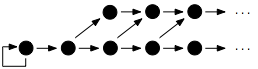
\includegraphics{../images/graphs/graf7_omega_w3.png}
		\caption{The $\beta$-reduction graph $G_\beta(\Omega w_3)$}
		\label{fig:images_graphs_graf7_omega_w3}
	\end{figure}
\end{example}
Note that these examples only serve to illustrate the \emph{structure} of a 
$\beta$-reduction graph, not the actual graph visualization that we develop
in this thesis.
%!TEX root = rapport.tex

\chapter{Existing visualizations in lambda theory}

There does not exist anything similar to what we are doing in this thesis.
However, there does exist many examples of projects making other types of
visualizations of the lambda calculus. In this section we will discuss these.

There are numerous examples of software with which a lambda term or a
reduction step for a lambda term can be visualized. We have found 7 examples
of such programs. For a complete list, see Appendix \ref{app:a}.
What differentiates these examples from this project are mainly two things:
\begin{itemize}
	\item
	In our project we focus on the reduction graphs, and not on
	the particular reductions, whereas the earlier work focus on
	visualizing either particular reduction steps or the syntactic structure
	of lambda terms. 
	
	\item
	None of the existing visualizations are in our opinion very good-looking.
\end{itemize}

In the rest of this chapter we will describe the two most interesting examples.

\section{Alligator Eggs -- A Puzzle Game by Bret Victor}

% \begin{figure}[h!]
% 	% \centering
% 		
\includegraphics[width=0.1in]{../images/AlligatorEggs.png}
% 	\caption{Alligator Eggs -  A Puzzle Game}
% 	\label{fig:images_AlligatorEggs}
% \end{figure}

The ``Alligator Eggs - A Puzzle Game'' \cite{Alligator} is a ``fun'' and
children-like way of visualizing $\beta$-reductions of a lambda term. It was
originally not intended to be a computer program; the author instead designed
a set of drawings meant to be printed and cut out. This way, the visualization
can be used as a game. It visualizes the syntactic structure of lambda
terms, and the allowed ``moves'' in the game correspond to $\alpha$-conversion or
$\beta$-reduction.

The game uses a simple graphical alphabet:
\begin{description}
	\item[A hungry alligator] represents a lambda abstraction. The symbol can
	have different colors, analogously to variable names in ordinary lambda calculus.
	\item[An old alligator] is a parenthesis. It can only be white.
	\item[An egg] is a variable. It, too, can take on different colors.
\end{description}
Alligators are organized vertically into ``families''. The different families
are organized horizontally next to each other, and they are guarded by either an
old or a hungry alligator. The old alligator only concerns itself with
guarding, while the hungry alligator also has one or more eggs associated. If
an alligator and an egg are associated with each other, they have the same
color. It is straightforward to see the analogy to lambda terms.

With this alphabet, the rules are defined as follows:
\begin{description}
	\item[The Eating Rule] states that the topmost hungry alligator of a family can
	eat the family in front of it. When it does this it dies, but the eaten family
	is resurrected in its entirety from all the eggs associated with the hungry, dead
	alligator. This rule corresponds to a $\beta$-reduction. 
	\item[The Color Rule] states, that if an eaten family contains alligators and eggs
	in the same color as some alligators or eggs in the eating family, these must change colors
	to some new, unused color. This rule corresponds to an $\alpha$-conversion.
	\item[The Old Age Rule] states, that if the topmost alligator of a family is
	an old alligator, this alligator may die and nothing will happen. This is in analogy
	to the convention, that outermost parentheses in lambda terms are removed.
\end{description}

In figure \ref{fig:images_alligatorEat} we can see the Eating Rule in use. The
green alligator will eat whatever is in front of it. In this case it will eat
the yellow alligator and its yellow egg. After the green alligator has eaten
the yellow alligator and egg, it will die and its egg will hatch into what it
has eaten. ``The miracle of life'', as the author calls it. This so-called
``miracle'' is in our profane terminology called a $\beta$-reduction, as
mentioned above.

% \begin{figure}[htbp]
% 	\centering
% 		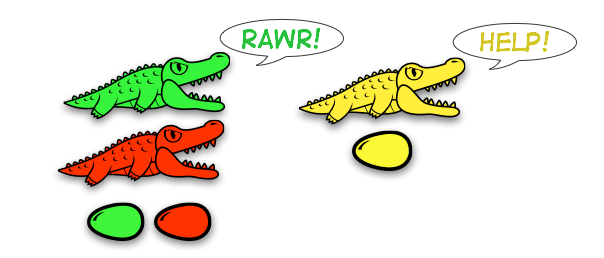
\includegraphics[width=2in]{../images/alligatorEat.png}
% 	\caption{A reduction visualized as an alligator eating}
% 	\label{fig:images_alligatorEat}
% \end{figure}

``Alligator Eggs - A Puzzle Game'' does not deal with the same kind of
visualization tasks that we do in this project. It basically presents a
creative way of drawing syntax trees and a new, carnivorous terminology for
the transformations in the lambda calculus. 

The game has been implemented as a Java program, so that one does not need to
actually print out the alligators. (\cite{AlligatorTool})

\section{Lambda Animator by Mike Thyer}
The ``Lambda Animator'' is a representation of lambda terms in tree
form. It is implemented in Java and available online via a Java Applet (\cite{lambdaAnimator}).
% \begin{figure}[!htbp]
% 	\centering
% 		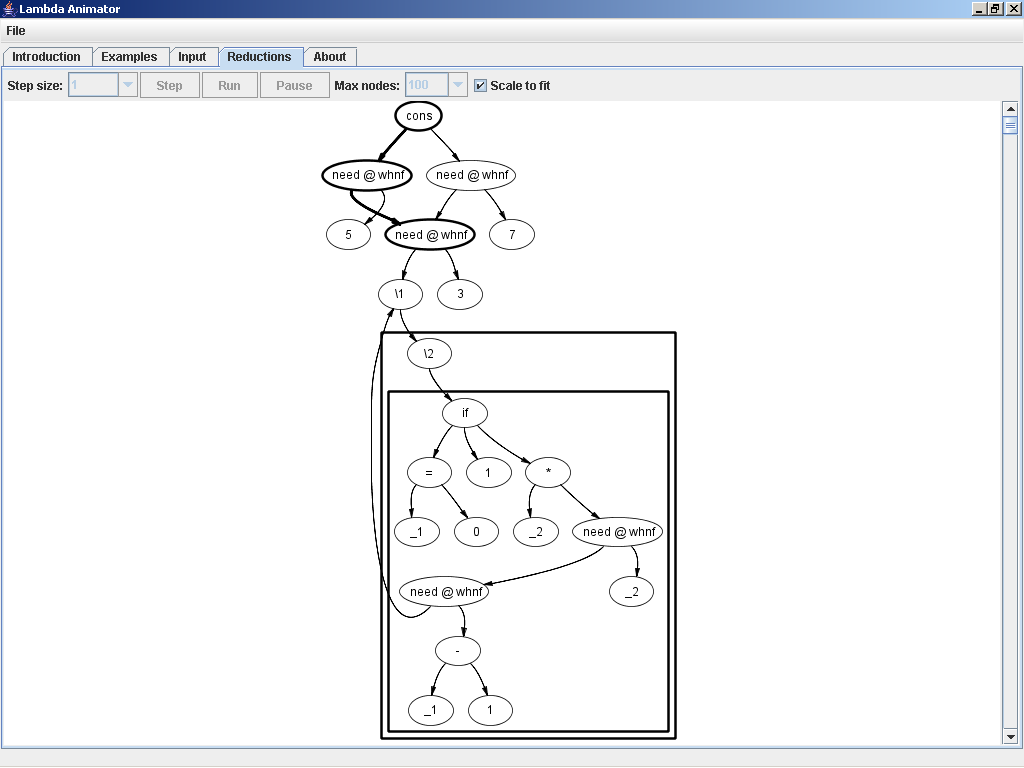
\includegraphics[scale=0.1]{../images/lambdaAnimator.png}
% 	\caption{Screenshot of the Lambda Annimator tool}
% 	\label{fig:images_lambdaAnimator}
% \end{figure}

The Animator does not seem very smooth and does not produce graphs that are
neither pretty nor especially visually informative. It uses extremely simple
graphics and does not fulfill our ``pretty'' criteria. The implementation in
the form of a Java applet does have some advantages in terms of easy access to
the tool.

It can give an reasonable overview when the lambda terms are not to complex.
In figure \ref{fig:images_lambdaAnimatorReduction} there is an example of a
simple $\beta$-reduction.
% \begin{figure}[!htbp]
% 	\centering
% 		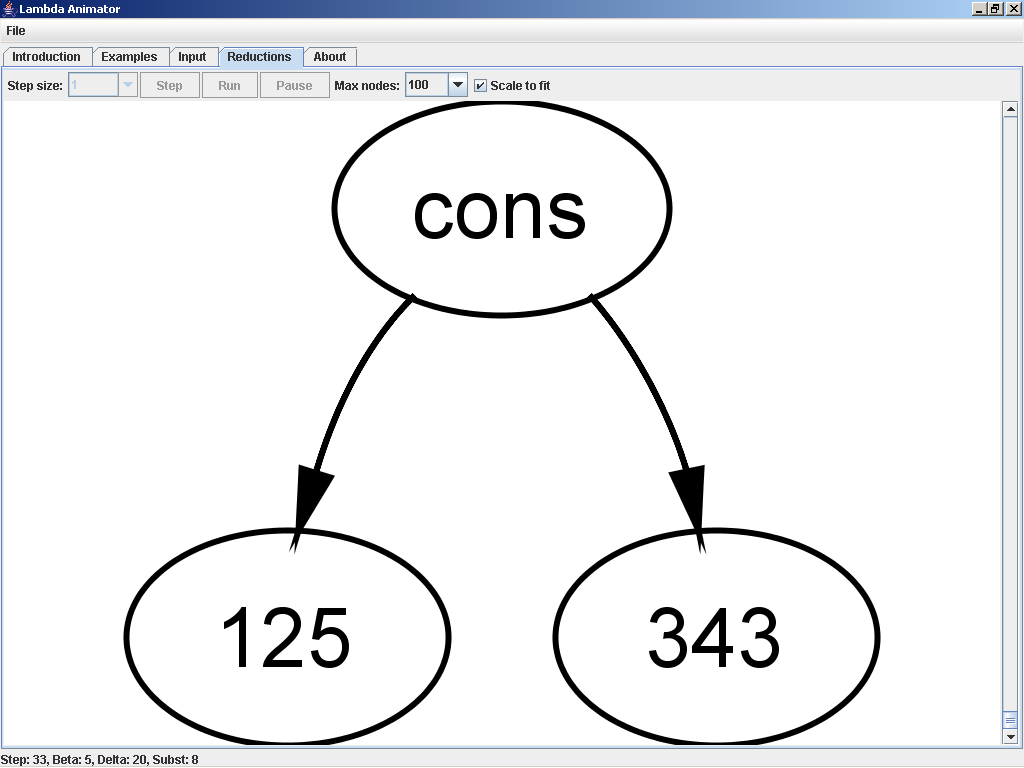
\includegraphics[scale=0.25]{../images/lambdaAnimatorReduction.png}
% 	\caption{Example of a simple $\beta$-reduction in the Lambda Animator}
% 	\label{fig:images_lambdaAnimatorReduction}
% \end{figure}

When you are dealing with more complex lambda terms it very easy gets chaotic.
In figure \ref{fig:images_lambdaAnimatorComplex} there is another example, in
which one can see that the informativeness seems to drastically degrade when
the term complexity is increasing.
% \begin{figure}[!htbp]
% 	\centering
% 		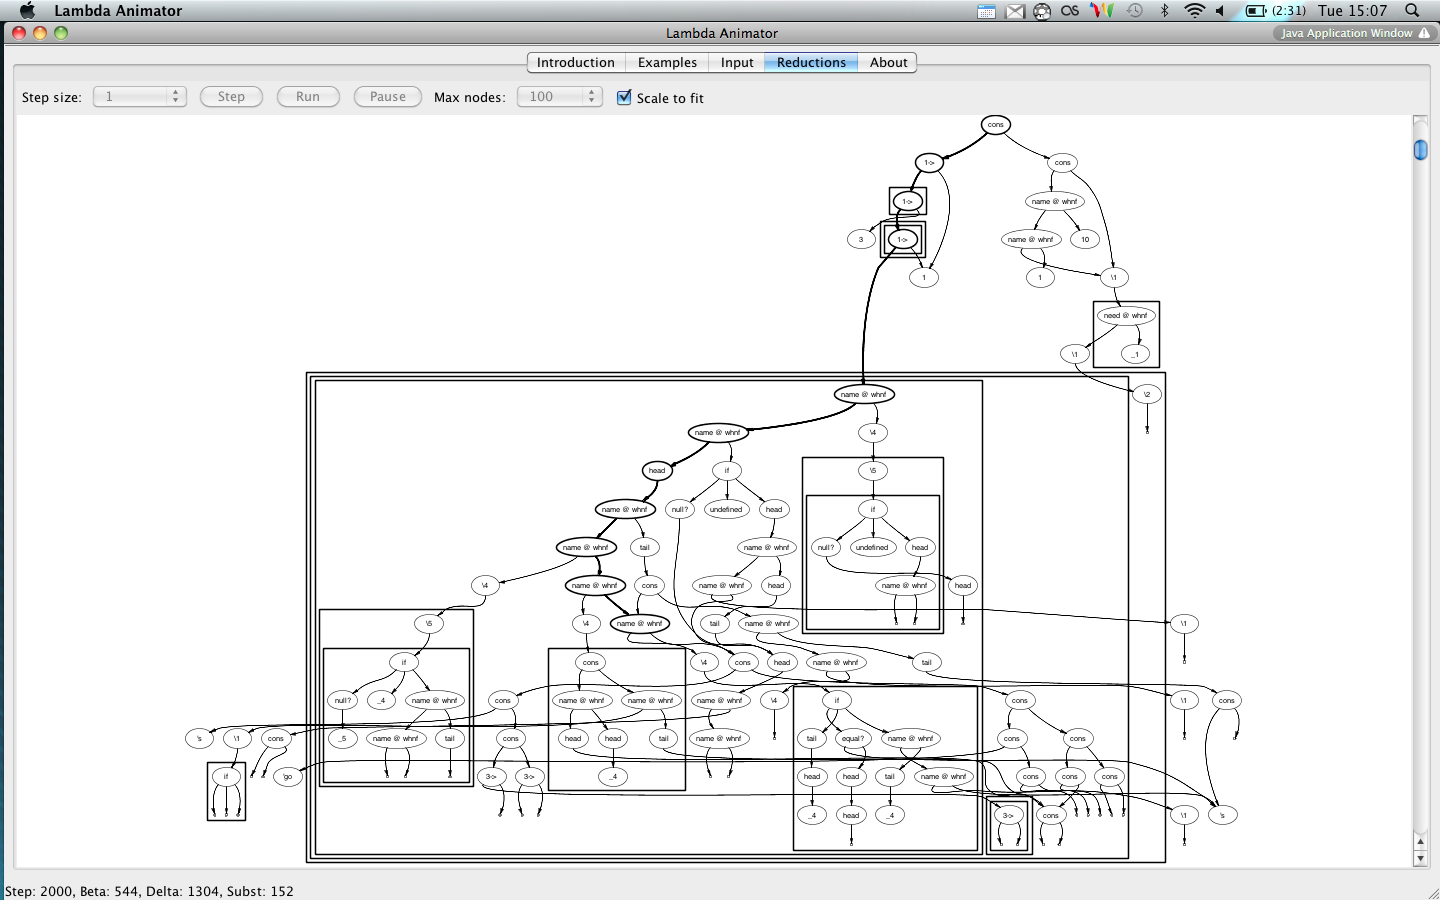
\includegraphics[scale=0.25]{../images/lambdaAnimatorComplex.png}
% 	\caption{Complex example in the Lambda Animator}
% 	\label{fig:images_lambdaAnimatorComplex}
% \end{figure}
%!TEX root = rapport.tex

\chapter{Representation of Lambda Terms in Python}

A lambda term is represented as a directed acyclic graph (DAG). The nodes of the
DAG are encoded in Python as objects. There are three types of nodes: 
abstraction, application and variable:
\begin{description}
	\item[Abstraction nodes] define scopes for bound variables and can be thought
	of as the encoding of the $\lambda$s in the DAG-structure. This node type
	always has one child.
	
	\item[Application nodes] have two children. The first of these
	is either the DAG-representation of some \emph{active} subterm of 
	$M$, or another application node. The second child is the DAG-representation
	of the ``argument'', that is, the lambda term that are to be substituted
	in place for a bound variable. An application node represents a possible
	one-step $\beta$-reduction.
	
	\item[Variable nodes] represent free or bound variables. A bound 
	variable is associated with a scope, represented by an ancestral
	abstraction node. Variable nodes cannot have descendants.
\end{description}

This representation is straightforwardly encoded in Python with a general node
class, \pycode{LambdaNode}, which has a subclass for each node type.
\begin{itemize}
	\item Each \pycode{LambdaNode}-object maintains pointers to its immediate 
	descendants as well as a pointer to its parent node.
	
	\item The abstraction nodes furthermore maintain a list of pointers to the
	variable nodes that represent the variables bound by this particular abstractor.
	These variable nodes must be descendants of the abstraction node, although 
	not necessarily direct descendants.
	
	\item Every abstraction node knows the name of the variable that it binds.
	This is done in order to be able to easily build the list of bound 
	variables after parsing a string representation of a lambda term. When
	the list of variables has been built, this name is not important anymore, 
	but it still serves as a means of producing human-readable output of the DAG.
	
	\item When a term is reduced, the problem is attacked ``top-down'', i.e. we first
	see the abstraction node, and then we have to deal with its variables.
	Therefore there is no need for a doubly linked connection between abstraction
	nodes and variable nodes, and we can safely encode the relationship as a simple
	list of bound nodes in each abstraction node.
\end{itemize}

A term that is not in $\beta$-normal-form has at least one $\beta$-contractum,
and therefore the DAG-representation of that term contains at least one
application node and one abstraction node. More specifically, for each
possible one-step $\beta$-reduction in a term $M$, its DAG will contain one
application node. The first descendant of this node will be an abstraction
node, while the second, ``rightmost'', descendant will be the argument that
will be applied to the function represented by the abstraction node.

Given this DAG, it is possible to implement the aforementioned operations on lambda
terms by treewalks. 


% Callback functions? Hvad skal de bruges til?


% \x.xy bliver til
%    L
%    |
%    @
%   / \ 
%  x   y


% application node: @
% abstraction node: L
% variable node: x,y..

% identify each of the possible reducts: find all active subterms.


% (\x.xx)(\y.\z.zyz) == (\x.xx)(\y.\z.(zy)z)
%        @
%       / \
%      L   ------L
%      |         |
%      @         @
%     / \       / \
%    x  x      @   z
%             / \
%            z   y
% .... or:
%       @
%      / \
%    Lx   Ly
%     |   |
%    xx   Lz
%         |
%         zyz

% (\x.xx)(\y.yy)(\z.zz) == ((\x.xx)(\y.yy)) (\z.zz)
%          @
%         / \
%        @   Lz
%       / \  |
%     Lx  Ly zz
%      |   | 
%     xx  yy 
% .... becomes:
%       @
%      / \
%     @   --- Lz
%    / \      |
%   Ly  Ly    zz
%   |   |
%   yy  yy
%

% I(Iz) -> Iz
% (\x.x)((\y.y)z) -> (\y.y)z
%          @
%         / \
%        Lx  ---@
%        |     / \
%        x    Ly  z
%             |
%             y
% indeholder to one-step betareductions:
%     @
%    / \
%   Ly  z
%   |
%   y
% og (ækvivalent!):
%     @
%    / \
%   Lx  z
%   |
%   x

%!TEX root = rapport.tex

\chapter{The parser and YAPPS2 parser generator}

This is about the parser.
%!TEX root = rapport.tex

\chapter{Graph Drawing}

% Polyline, straightline, orthogonal drawings.
% Use a graphic standard to define elements of the graph drawing.
% Aesthetics: distance between adjacent nodes, minimum bounding box, crossing edges,
%			symmetries, bendings of edges, uniform edge lengths, uniform vertex distribution.
% Aesthetics are in general NP-hard.
% Aesthethics are often "competitive" -- optimality of one means suboptimality of another one.
% "Spring algorithms": Edges are springs and vertices are rings. (gdbiblio: 43)
% 	http://en.wikipedia.org/wiki/Force-based_algorithms
% Simulated annealing approach; uses an energy function. (gdbiblio: 50)
% Mixture of different heuristics presented in (gdbiblio: 52).

% Non-planarity: Make non-planar graphs planar (gdbiblio: 55) "planarization"
% Find the maximum, planar subgraph (NP-hard) or find a small number of edges to delete
%	in order to make the graph planar. (gdbiblio 55-66) Or find subgraph with minimum number
%	of crossings (NP-hard) (gdbiblio 67).
%	Or one can split the graph to planarize it (gdbiblio: 68)

% Automatic layout of orthogonal grid drawings graphs (gdbiblio 72,73)
%	Allow homogenous treatment w/ same aesthetics of a wide range of graphs.

% To draw a non-planar graph: planarize it and apply planar drawing algorithm.
% Draw: 
%	Test planarity of graph (gdbiblio: 78-83)
%	Construct planar representation (gdbiblio: 84)
%	Planar representation with drawing algorithm.
% Every planar graph can be drawn as a planar straightline graph (gdbiblio: 85-87)
% Convex drawings are planar straightline drawings where every face is drawn as 
%	a convex polygon (gdbiblio: 89,90)
% Minimize the line length in a straightline planar drawing with a convex boundary (gdbiblio: 94,95)
% O(n) algorithm for drawing planar straightline: (gdbiblio: 97)
% Display symmetries in planar straightline drawings: (gdbiblio: 98-101)
% Every planar graph can be drawn as planar straightline grid drawing with area O(n^2) (gdbiblio: 102-104)
% Different planar graph drawing algorithms are compared in (gdbiblio: 106)

% Orthogonal grid drawings were motivated by circuit layout.
% Aesthetic: minimize the area and the number of bends.
% Every planar graph (degree at most 4) can be drawn as a planar orthogonal 
%	grid layout with area O(n^2) 
% It is NP-hard to test whether a planar graph can be drawn orthogonally without bends (gdbiblio: 112)
%	and it is NP-hard to minimize the number of bends!
% Minimize the number of bends in O(n^2log n) in an embedded setting (gdbiblio: 113)
% Heurstics for drawing orthogonal grid drawings with O(n) bends in (gdbiblio: 115)
% Survey of orthogonal drawing algorithms in (gdbiblio: 122)

% Visibility representations: represent each vertex as a horisontal line and each 
%	edge as a horisontal line. The edge lines intersects exactly those two vertices
%	that the connect. (gdbiblio: 124)
% Algorithms for constructing visiility representations in linear time given in (gdbiblio: 132-136)







% Hvad _er_ det at "tegne" en graf?
%	Det er en projektion af en graf G(V,E) på planet, således at hver
%	knude i V er repræsenteret ved et grafisk symbol, og så der mellem
%	alle tegnene for knuder (V_1,V_2)\in E er et linjestykke...

% Hvilke problemer støder man på når man tegner en graf?
%	Hvordan skal knuderne placeres?
%	Hvordan undgår man at kanter overlapper?
%	Hvor store skal knuderne være?
%	Hvad skal bruges som pile?
%	Når en ikke-planar graf tegnes, hvordan mindsker man antallet af overlap?
%		Er der et teoretisk minimum evt.?
%	Er der mange der begynder at tegne i tre dimensioner som en løsning?
%		Enhver graf kan realiseret uden overlap i 3D (se DujomovicWood).
%	Hvordan repræsenterer folk de krydsninger der uundgåeligt kommer i visse
%	grafer?
%	Hvordan ser det ud mht. størrelsesforholdet mlm. kanter og knuder?


% Hvordan udregner folk afstanden mlm. knuderne?

% Hvordan håndterer folk problemet med non-planaritet?
%   "Confluent Drawings.."-solution
%    3-dimensional drawing: "Three-Dimensional Grid Drawings with Sub-quadratic Volume⋆"

% Hvordan tegner folk pilehovederne i en retningsbestemt graf?

% Hvordan anvender folk farver i graftegningen?

% Hvilke programmer til tegning af grafer eksisterer der?



% Planarity problems:
%   "Confluent Drawings.."-solution
%    3-dimensional drawing: "Three-Dimensional Grid Drawings with Sub-quadratic Volume⋆"

% G. Di Battista, P. Eades, R. Tamassia, and I. G. Tollis, 
%   Graph Drawing, Prentice Hall, Upper Saddle River, NJ, 1999.

% Pilehoveder?



% Appendices

%\appendix
% %!TEX root = rapport.tex

\chapter{First appendix}\label{app:a}

% %!TEX root = rapport.tex

\chapter{Next appendix}\label{app:b}
%%!TEX root = rapport.tex

\chapter{And the following}\label{app:c}
%
% Bibliography
\bibliographystyle{abbrv}
\bibliography{bibliography,bibl_graph_drawing}



%%%%%%%%%%%%%%%%%%%%%%%%%%%%%%%%%%%%%%%%%%%%%%%%%%
\end{document}
%%%%%%%%%%%%%%%%%%%%%%%%%%%%%%%%%%%%%%%%%%%%%%%%%%
